% vim:syntax=tex

In this section we describe the design of a case study in which we
compare topic models trained on changesets to those trained on snapshots.
%explore the relationship between ownership and linguistic topics in source code.
We describe the case study using the Goal-Question-Metric approach~\cite{Basili-etal:94}.
% TODO
%The data for the case study is available in this paper's online
%appendix\footnote{\url{xxxxxx}}.

\subsection{Definition and Context}

% TODO
Our \textit{goal} is to ... 
The \textit{quality focus} of the study is on informing development
decisions and policy changes that could lead to software with fewer
defects.
The \textit{perspective} of the study is of a researcher, developer, or
project manager who wishes to gain understanding of the concepts or
features implemented in the source code.
The \textit{context} of the study spans the version histories of ...
open source systems.

Toward achievement of our goal, we pose the following research questions:
\begin{description}[font=\itshape\mdseries,leftmargin=10mm,style=sameline]
% TODO
    \item[RQ1] .... 
\end{description}
At a high level, we want to...
In the remainder of this section we introduce the subjects of our study,
describe the setting of our study, and report our data collection and analysis procedures.

%%%%%%%%%%%%%%%%%%%%%%%%%%%%%%%%%%%%%%%%%%%%%%%%%%%%%%%%%%%%%%%%%%%%%%%%

\subsection{Subject software systems}

% TODO

%%%%%%%%%%%%%%%%%%%%%%%%%%%%%%%%%%%%%%%%%%%%%%%%%%%%%%%%%%%%%%%%%%%%%%%%

\subsection{Setting}

\begin{figure*}[!th]
    \centering
    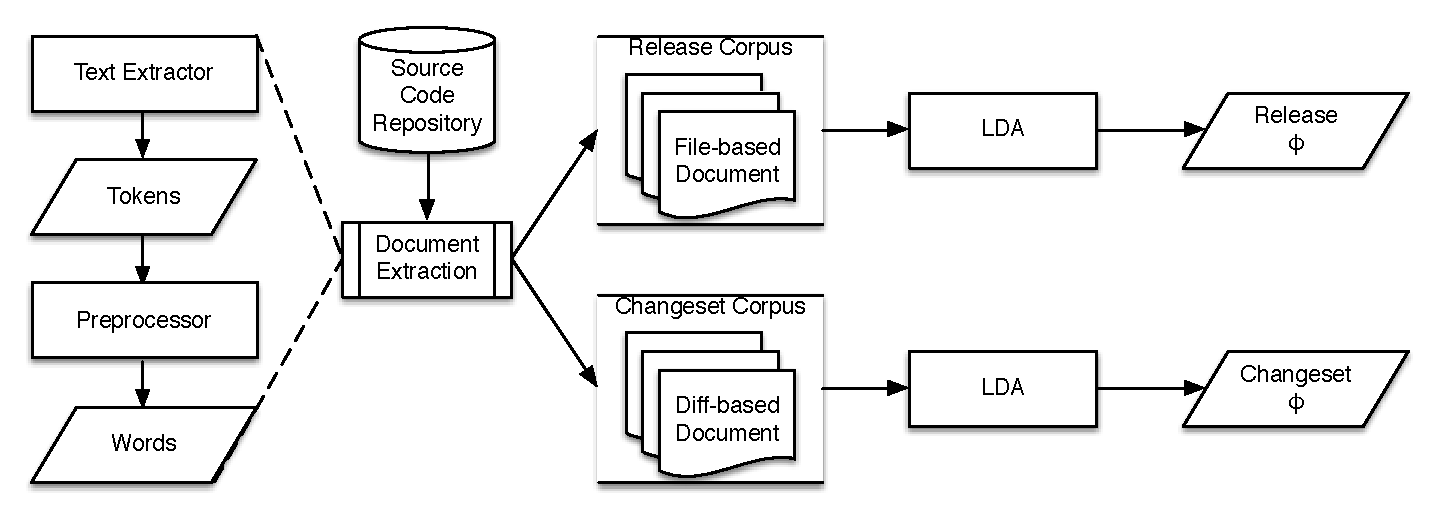
\includegraphics[width=.75\textwidth]{changeset}
    \caption{Extraction and Modeling Process}
    \label{fig:process}
\vspace{-10pt}
\end{figure*}

Our document extraction process is shown on the left side of Figure~\ref{fig:process}.
We implemented our document extractor in Python v2.7
using the Dulwich library\footnote{\url{http://www.samba.org/~jelmer/dulwich/}}. %\footnote{\url{https://pypi.python.org/pypi/dulwich}}
We extract documents from both a snapshot of the repository at a tagged
release and each commit reachable from that tag's commit.
The same preprocessing steps are employed on all documents extracted.

% TODO
For our document extraction from a snapshot, we ...

To extract text from the changesets, we look at the output of viewing
the \texttt{git diff} between two commits.
Figure~\ref{fig:diff} shows an example of what a changeset might look
like in Git.
In our changeset text extractor, we only extract all text related to the
changed file, e.g., context, removed, and added lines.  
Metadata lines are ignored.
Note that we do not consider where the text originates from,
only that it is text changed by the commit.

After extracting tokens, we split them based on camel case, underscores, and non-letters.
We normalize to lower case before filtering non-letters, English stop words~\cite{StopWords}, Java keywords, and words shorter than three characters long.
We do not stem words.

Our modeling generation is shown on the right side of Figure~\ref{fig:process}.
We implemented our modeling using the Python library Gensim~\cite{Gensim}.
Gensim's LDA implementation is based on an Online LDA by Hoffman et al.~\cite{Hoffman-etal:2010}
and uses variational inference instead of a Collapsed Gibbs Sampler.
Unlike Gibbs sampling, in order to ensure that the model converges for each document,
we allow LDA to see each document $10$ times by setting Gensim's initialization parameter \texttt{passes} to this value.
% TODO
We set the following LDA parameters for all ... systems:
$100$ topics ($K$),
a symmetric $\alpha=0.01$,
$\beta$ is left as a default value of $1/K$ (also $0.01$).


\begin{figure}[ht]
\centering
\footnotesize
\begin{lstlisting}[language=diff, basicstyle=\ttfamily]
diff --git a/lao b/tzu
index 635ef2c..5af88a8 100644
--- a/lao
+++ b/tzu
@@ -1,7 +1,6 @@
-The Way that can be told of is not the eternal Way;
-The name that can be named is not the eternal name.
 The Nameless is the origin of Heaven and Earth;
-The Named is the mother of all things.
+The named is the mother of all things.
+
 Therefore let there always be non-being,
   so we may see their subtlety,
 And let there always be being,
@@ -9,3 +8,6 @@ And let there always be being,
 The two are the same,
 But after they are produced,
   they have different names.
+They both may be called deep and profound.
+Deeper and more profound,
+The door of all subtleties!
\end{lstlisting}
\caption{Example of a \texttt{git diff}. Black or blue lines denote metadata about the change useful for patching, red lines (beginning with a single~\texttt{-}) denote line removals, and green lines (beginning with a single~\texttt{+}) denote line additions.}
\label{fig:diff}
\vspace{-10pt}
\end{figure}


%%%%%%%%%%%%%%%%%%%%%%%%%%%%%%%%%%%%%%%%%%%%%%%%%%%%%%%%%%%%%%%%%%%%%%%%

\subsection{Data Collection and Analysis}

% TODO
We create two corpora for each of our four subject systems.
We then used LDA to model the documents into topics.

To answer RQ1, ... 


%%%%%%%%%%%%%%%%%%%%%%%%%%%%%%%%%%%%%%%%%%%%%%%%%%%%%%%%%%%%%%%%%%%%%%%%

\subsection{Results}

% TODO
RQ1 asks ...
